\section{Method}\label{sec:method}
Fig.~\ref{fig:pipeline} gives an overview. Each partition maintains a sketch of the signatures it has seen in the current window. At the end of the window the sketches are merged and compared with the merged sketch of the previous window.

\begin{figure}[t]
  \centering
  % Replace with your own figure: upload an image and change the file name below.
  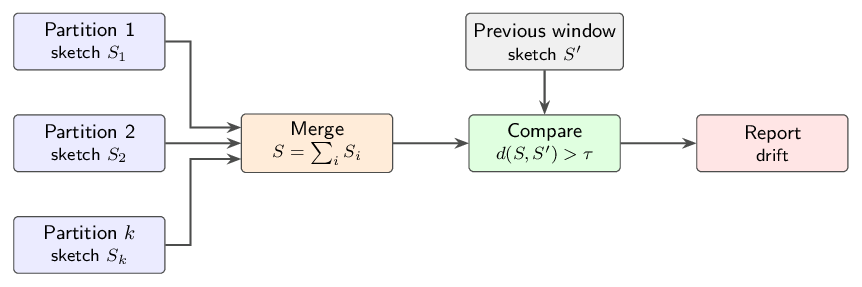
\includegraphics[width=0.95\textwidth]{figures/pipeline.png}
  \caption{Stages of the detector. Sketches are built per partition, merged per window, and compared with the previous window; a difference above the threshold raises a report.}
  \label{fig:pipeline}
\end{figure}

\subsection{The Sketch}
The sketch is an array $S$ of $m$ counters. For every pair $(p, t)$ in a record's signature we increment $S[h(p, t)]$, where $h$ maps pairs to $\{1, \dots, m\}$ uniformly. We also count the number of records $n$. Two sketches with the same $m$ and $h$ are merged by adding their arrays and their record counts, which is associative and commutative.

\subsection{Comparing Windows}
Let $S$ and $S'$ be the sketches of two consecutive windows with $n$ and $n'$ records. We compare the relative frequencies of the counters,
\begin{equation}\label{eq:distance}
  d(S, S') = \max_{1 \le j \le m} \left| \frac{S[j]}{n} - \frac{S'[j]}{n'} \right| ,
\end{equation}
and report drift when $d(S, S') > \tau$ for a threshold $\tau$. Algorithm~\ref{alg:detect} summarizes the procedure.

\begin{algorithm}[t]
\caption{Drift detection for one window}
\label{alg:detect}
\begin{algorithmic}[1]
\Require records $R_1, \dots, R_k$ of the $k$ partitions; previous sketch $S'$ with count $n'$; threshold $\tau$
\Ensure \textsc{true} if drift is detected
\For{$i \gets 1$ \textbf{to} $k$} \Comment{in parallel}
  \State $S_i \gets \mathbf{0}$; $n_i \gets 0$
  \ForAll{records $r \in R_i$}
    \ForAll{$(p, t) \in \Call{Signature}{r}$}
      \State $S_i[h(p, t)] \gets S_i[h(p, t)] + 1$
    \EndFor
    \State $n_i \gets n_i + 1$
  \EndFor
\EndFor
\State $S \gets \sum_i S_i$; $n \gets \sum_i n_i$ \Comment{merge}
\State \Return $d(S, S') > \tau$
\end{algorithmic}
\end{algorithm}

\subsection{Guarantee}
A change is \emph{$\varepsilon$-significant} if it alters the presence or type of some field in at least a fraction $\varepsilon$ of the records of a window.

\begin{theorem}\label{thm:bound}
Let $\tau = \varepsilon / 2$ and let both windows contain at least $n$ records. An $\varepsilon$-significant change is reported with probability at least $1 - 2\exp(-n \varepsilon^2 / 8) - 1/m$.
\end{theorem}

\begin{proof}[Sketch]
The changed pair occupies some counter $j$. With probability at least $1 - 1/m$ no pair with an opposite change of the same size shares that counter, so the expected relative frequencies of counter $j$ differ by at least $\varepsilon$. By Hoeffding's inequality each observed frequency lies within $\varepsilon / 4$ of its expectation with probability at least $1 - \exp(-n \varepsilon^2 / 8)$, and a union bound over the two windows gives the claim. \qed
\end{proof}

With $m = 1200$ counters of two bytes each, the sketch occupies 2.4~kB, and for $n = 10^5$ and $\varepsilon = 0.02$ the bound exceeds 0.98.
